\section{Double homodyne detection scheme}\label{sec-double-homodyne}

Consider the 8-port double homodyne scheme (Fig.~\ref{fig:double-homodyne}) \cite{lahti2010realistic}. It is known that this measurement scheme allows to reconstruct the $Q$-function of the signal state \cite{Richter:98}, yielding full information about the signal state, which may be used in CV-QKD protocols. It should be noted that the restoration of the state complex amplitude entirely serves as the basis for composable security proofs~\cite{PhysRevLett.93.170504,PhysRevLett.118.200501,pirandola2024improvedcomposablekeyrates,pascualgarcía2024improvedfinitesizekeyrates}. Analogous to Eq.~\eqref{eq:accurate}, the statistical distribution of photon count difference is written as:
\begin{multline}
P= \left(\frac{\eta_1|\alpha_1|^2}{\eta_4|\alpha_4|^2}\right)^{\frac{\delta m_1}{2}}
I_{\delta m_1}\left(2\sqrt{\eta_1\eta_4|\alpha_ 1|^2|\alpha_4|^2}\right)
e^{-\eta_1|\alpha_1|^2}
e^{-\eta_4|\alpha_4|^2}\times\\\times
\left(\frac{\eta_3|\alpha_3|^2}{\eta_2|\alpha_2|^2}\right)^{\frac{\delta m_2}{2}}
I_{\delta m_2}\left(2\sqrt{\eta_2\eta_3|\alpha_ 2|^2|\alpha_3|^2}\right)
e^{-\eta_2|\alpha_2|^2}
e^{-\eta_3|\alpha_3|^2}\label{eq:accurate-dh},
\end{multline}
where
\begin{align}
\begin{split}
    |\alpha_1|&=|
    C_1C_2\alpha
    -S_3S_2\alpha_L|,\\
    |\alpha_2|&=
    |S_1C_4\alpha
    -iC_3S_4\alpha_L|,\\
    |\alpha_3|&=|
     S_1S_4\alpha
    +iC_3C_4\alpha_L|,\\
    |\alpha_4|&=|
    C_1S_2\alpha+
    S_3C_2\alpha_L|.
\end{split}
\end{align}

The approximation method used in the previous section yields the Gaussian approximation
\begin{multline}
P_G=\frac{\biggl[(\eta_1S_2^2+\eta_4C_2^2)(\eta_3C_4^2+\eta_2S_4^2)\biggr]^{-\frac{1}{2}}}{2\pi C_3S_3|\alpha_L|^2}\times\\\times \exp \biggl[-D_1\left(x_1+\frac{\Re\alpha\alpha_L^*}{|\alpha_L|}\right)^2\biggr]\exp \biggl[-D_2\biggl(x_2-\frac{\Im\alpha\alpha_L^*}{|\alpha_L|}\biggr)^2\biggr], \label{eq:Pgood-dh}
\end{multline}
where designations
\begin{align}
    \begin{split}
D_1&=\frac{2(C_1C_2S_2[\eta_1+\eta_4])^{2}}{\eta_1S_2^2+\eta_4C_2^2},\\
    D_2&=\frac{2(S_3S_4C_4[\eta_3+\eta_2])^2}{\eta_3C_4^2+\eta_2S_4^2},
    \end{split}\label{eq:dh-D}
\end{align}
\begin{align}
    \begin{split}
x_1&=\frac{\delta m_1}{2|\alpha_L|C_1C_2S_2S_3[\eta_1+\eta_4]}+\frac{-\eta_1S_2^2S_3^2+\eta_4S_3^2C_2^2}{2C_1C_2S_2S_3[\eta_1+\eta_4]}|\alpha_L|, \\
    x_2&=\frac{\delta m_2}{2|\alpha_L|S_1S_4C_3C_4[\eta_3+\eta_2]}+\frac{-\eta_3C_3^2C_4^2+\eta_2C_3^2S_4^2}{2S_1S_4C_3C_4[\eta_3+\eta_2]}|\alpha_L|
    .
    \end{split}\label{eq:dh-x}
\end{align}
have been introduced. Note that Eq.~\eqref{eq:Pgood-dh} is a product of two functions in the form of Eq.~\eqref{eq:Pgood} (much like Eq.~\eqref{eq:accurate-dh} is a product of two function in the form of Eq.~\eqref{eq:accurate}), meaning approximation quality study in previous section fully applies for this case. Indeed, the difference statistics of the double homodyne scheme is difference statistics of two separate homodyne schemes with quadrature displaced by $\frac{\pi}{2}$, normalized to unity (See Fig.~\ref{fig:dh-statistics}). 

Using the method introduced in the previous section, by comparing Eq.\eqref{eq:Pgood-dh} of the ideal scheme and the $Q$-function of coherent state,
\begin{equation}
    |\langle\beta|\alpha\rangle|^2=\exp\left[-
    (\beta_1-\alpha_1)^2-(\beta_2-\alpha_2)^2
    \right], %ez 2 show
\end{equation}
where for complex numbers we introduced the notation $\alpha=\alpha_1+i\alpha_2$, and introducing 
\begin{align}
\begin{split}
    \sigma_{D_1}\equiv\frac{1}{D_1}-1,\\
    \sigma_{D_2}\equiv\frac{1}{D_2}-1,
\end{split}
\label{eq:dh-G}
\end{align}
we may write $P_G$ in the form
\begin{multline}
    {{P}}_G=\frac{1}{4{\pi}C_3S_3[\eta_1+\eta_4][\eta_3+\eta_2]S_2^2\sqrt{ C_1C_2S_4C_4}|\alpha_L|^2} \int \mathop{dx'_1dx'_2}\times\\\times G(x_1-x_1', \sigma_{D_1})G(x_2-x_2', \sigma_{D_2})|\langle\alpha|e^{-i\phi_L}\left(-x_1'+ix_2'\right)\rangle|^2,%\label{eq:dh-povm}
\end{multline}
where $|e^{-i\phi_L}\left(-x_1'+ix_2'\right)\rangle$ is a coherent state. This allows us to write the respective POVM as
\begin{multline}
    \hat{{P}}_G=\frac{1}{4{\pi}C_3S_3[\eta_1+\eta_4][\eta_3+\eta_2]S_2^2\sqrt{C_1C_2S_4C_4}|\alpha_L|^2} \int \mathop{dx'_1dx'_2}\times\\\times G(x_1-x_1', D_1)G(x_2-x_2', D_2)|e^{-i\phi_L}\left(-x_1'+ix_2'\right)\rangle\langle e^{-i\phi_L}\left(-x_1'+ix_2'\right)|.\label{eq:dh-povm}
\end{multline}
Note the difference between definitions of variances of Gaussian functions Eq.~\eqref{eq:h-G} and Eq.~\eqref{eq:dh-G}, namely the difference in variances by a factor of $2$. This is due to $Q$-functions with which we compare approximations with ideal parameters having (and not having) an explicit factor of $2$ in their variances.

We may also see that $D_1$ and $D_2$, defined by Eq.~\eqref{eq:dh-D}, may be greater than $1$ for some parameters of the system. This becomes apparent once we present $D_1$ ($D_2$) as $2C_1^2D$ ($2S_3^2D$), with $D$ defined as per Eq.~\eqref{eq:defs-x-D}. This is an issue due to the variances $\sigma_{D_1}$ and $\sigma_{D_2}$ given by Eq.~\eqref{eq:dh-G}, being negative for these parameters, meaning that any asymmetry in BS$_1$ and BS$_3$ is not described by POVM given by Eq.~\eqref{eq:dh-povm}. \hl{Evidently, using coherent states for this case is flawed, see Ref.{~\cite{doi:10.1080/09500348714550131}}, where, for similar case of non-balanced BS$_{1,3}$, POVM is derived to be a projector onto squeezed coherent state.} This problem requires further investigation and is beyond the scope of this work.

\begin{figure}
    \centering
    \begin{minipage}[c]{.75\linewidth}
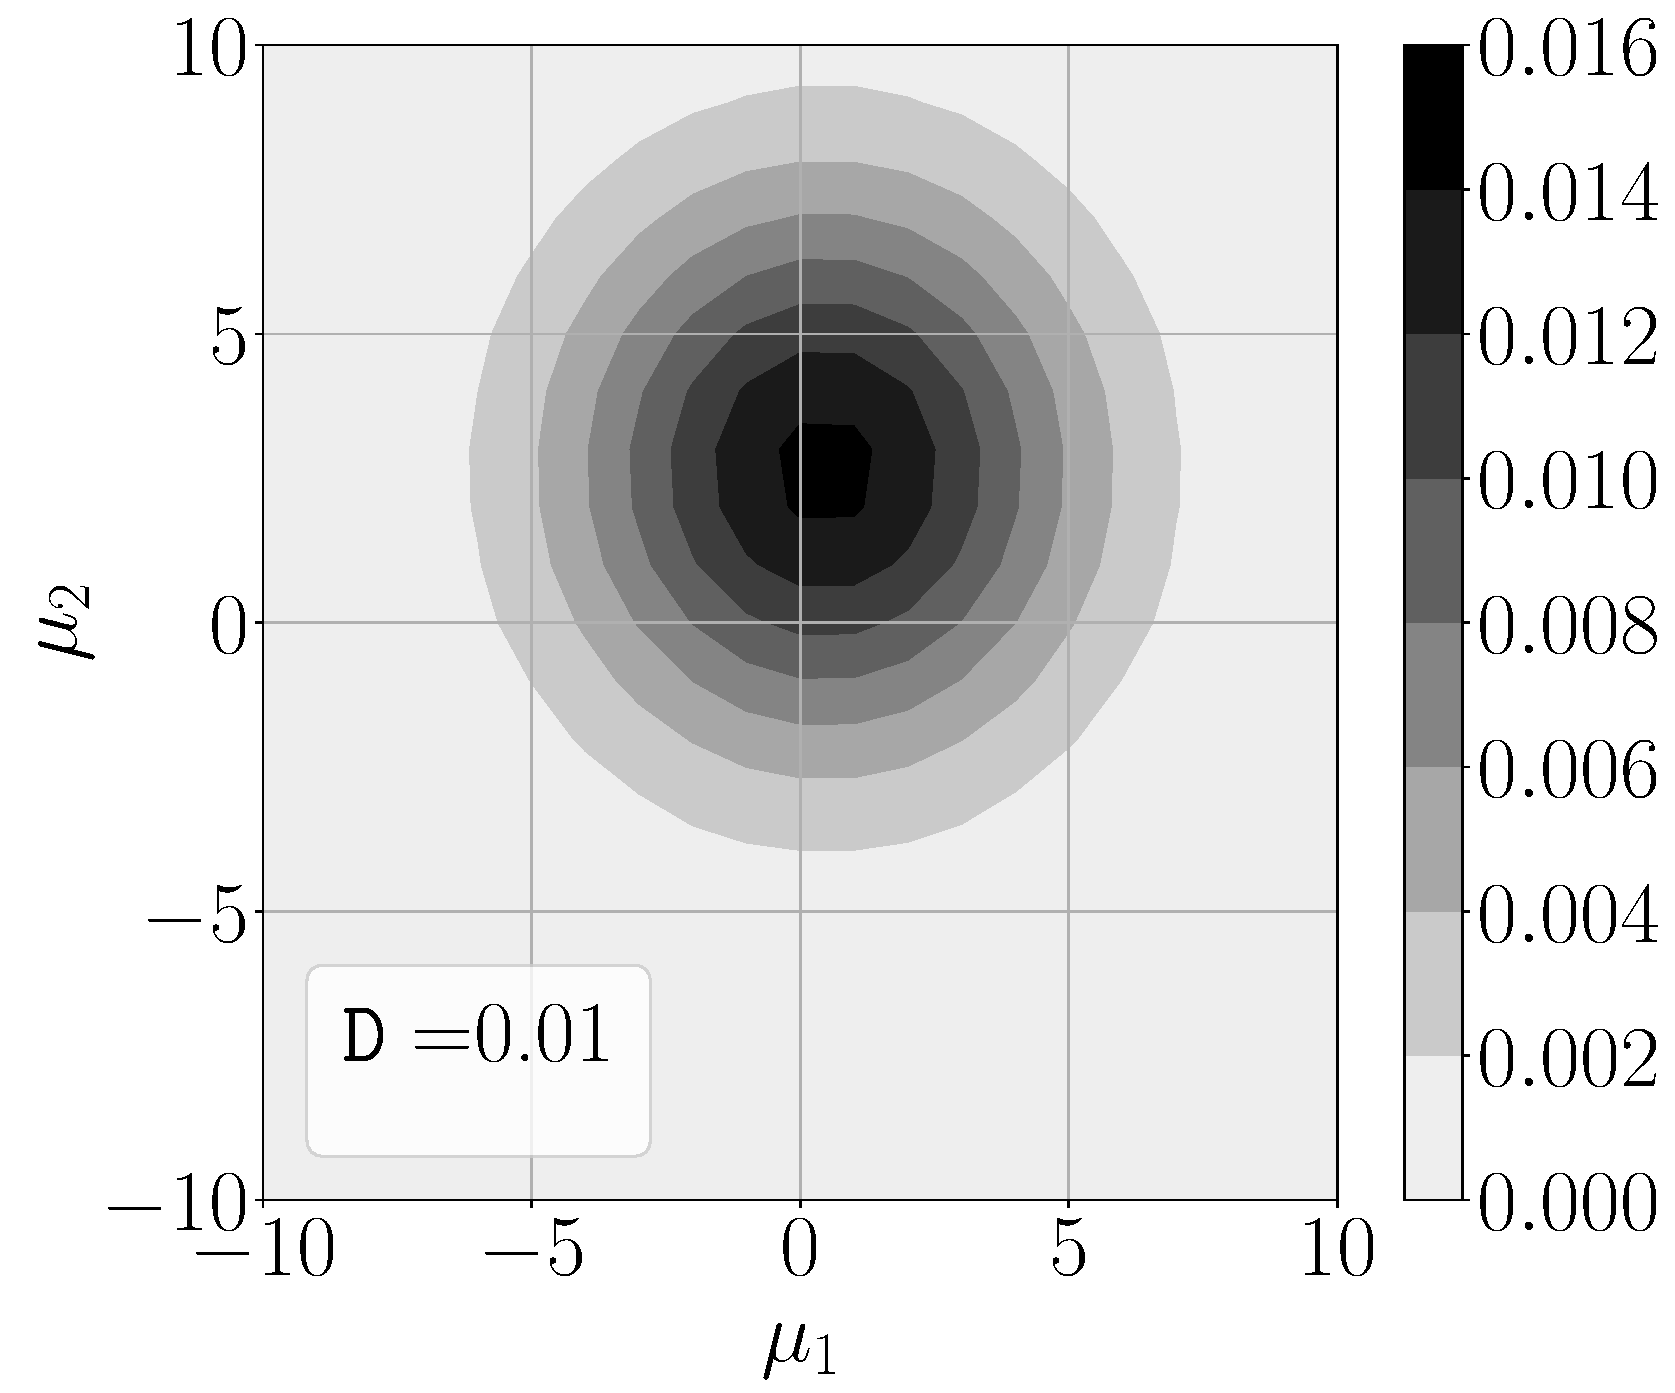
\includegraphics[width=\linewidth]{pics/double-homodyne/full.pdf}
\subcaption[]{}
        \end{minipage}
\hfill
        \begin{minipage}[c]{.45\linewidth}
 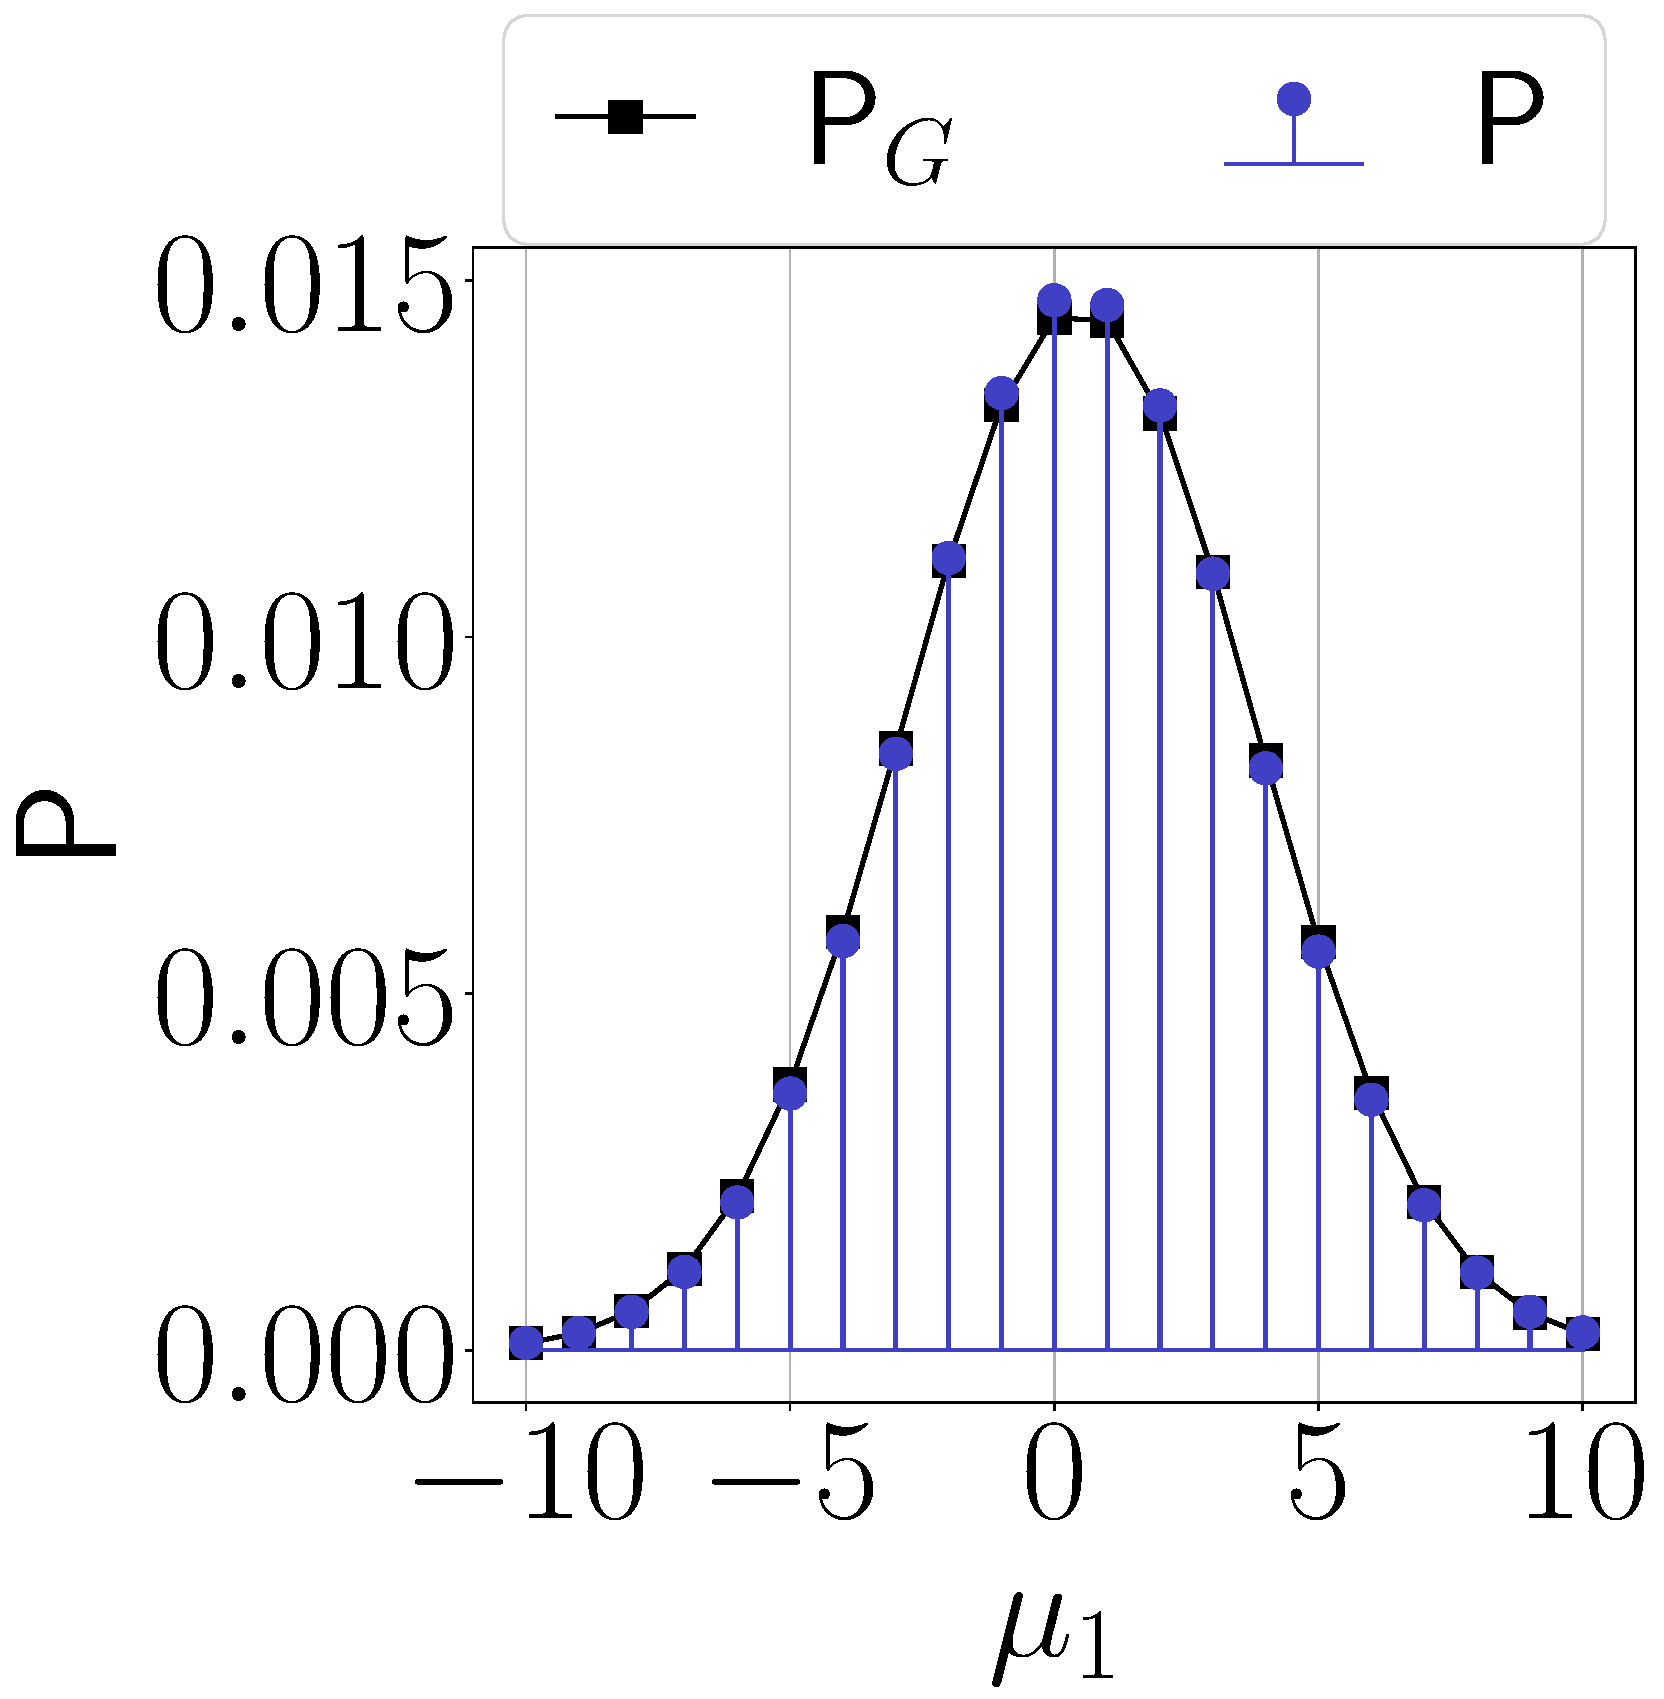
\includegraphics[width=\linewidth]{pics/double-homodyne/dm1.pdf}
\subcaption[]{}
\end{minipage}
\hfill
        \begin{minipage}[c]{.45\linewidth}
 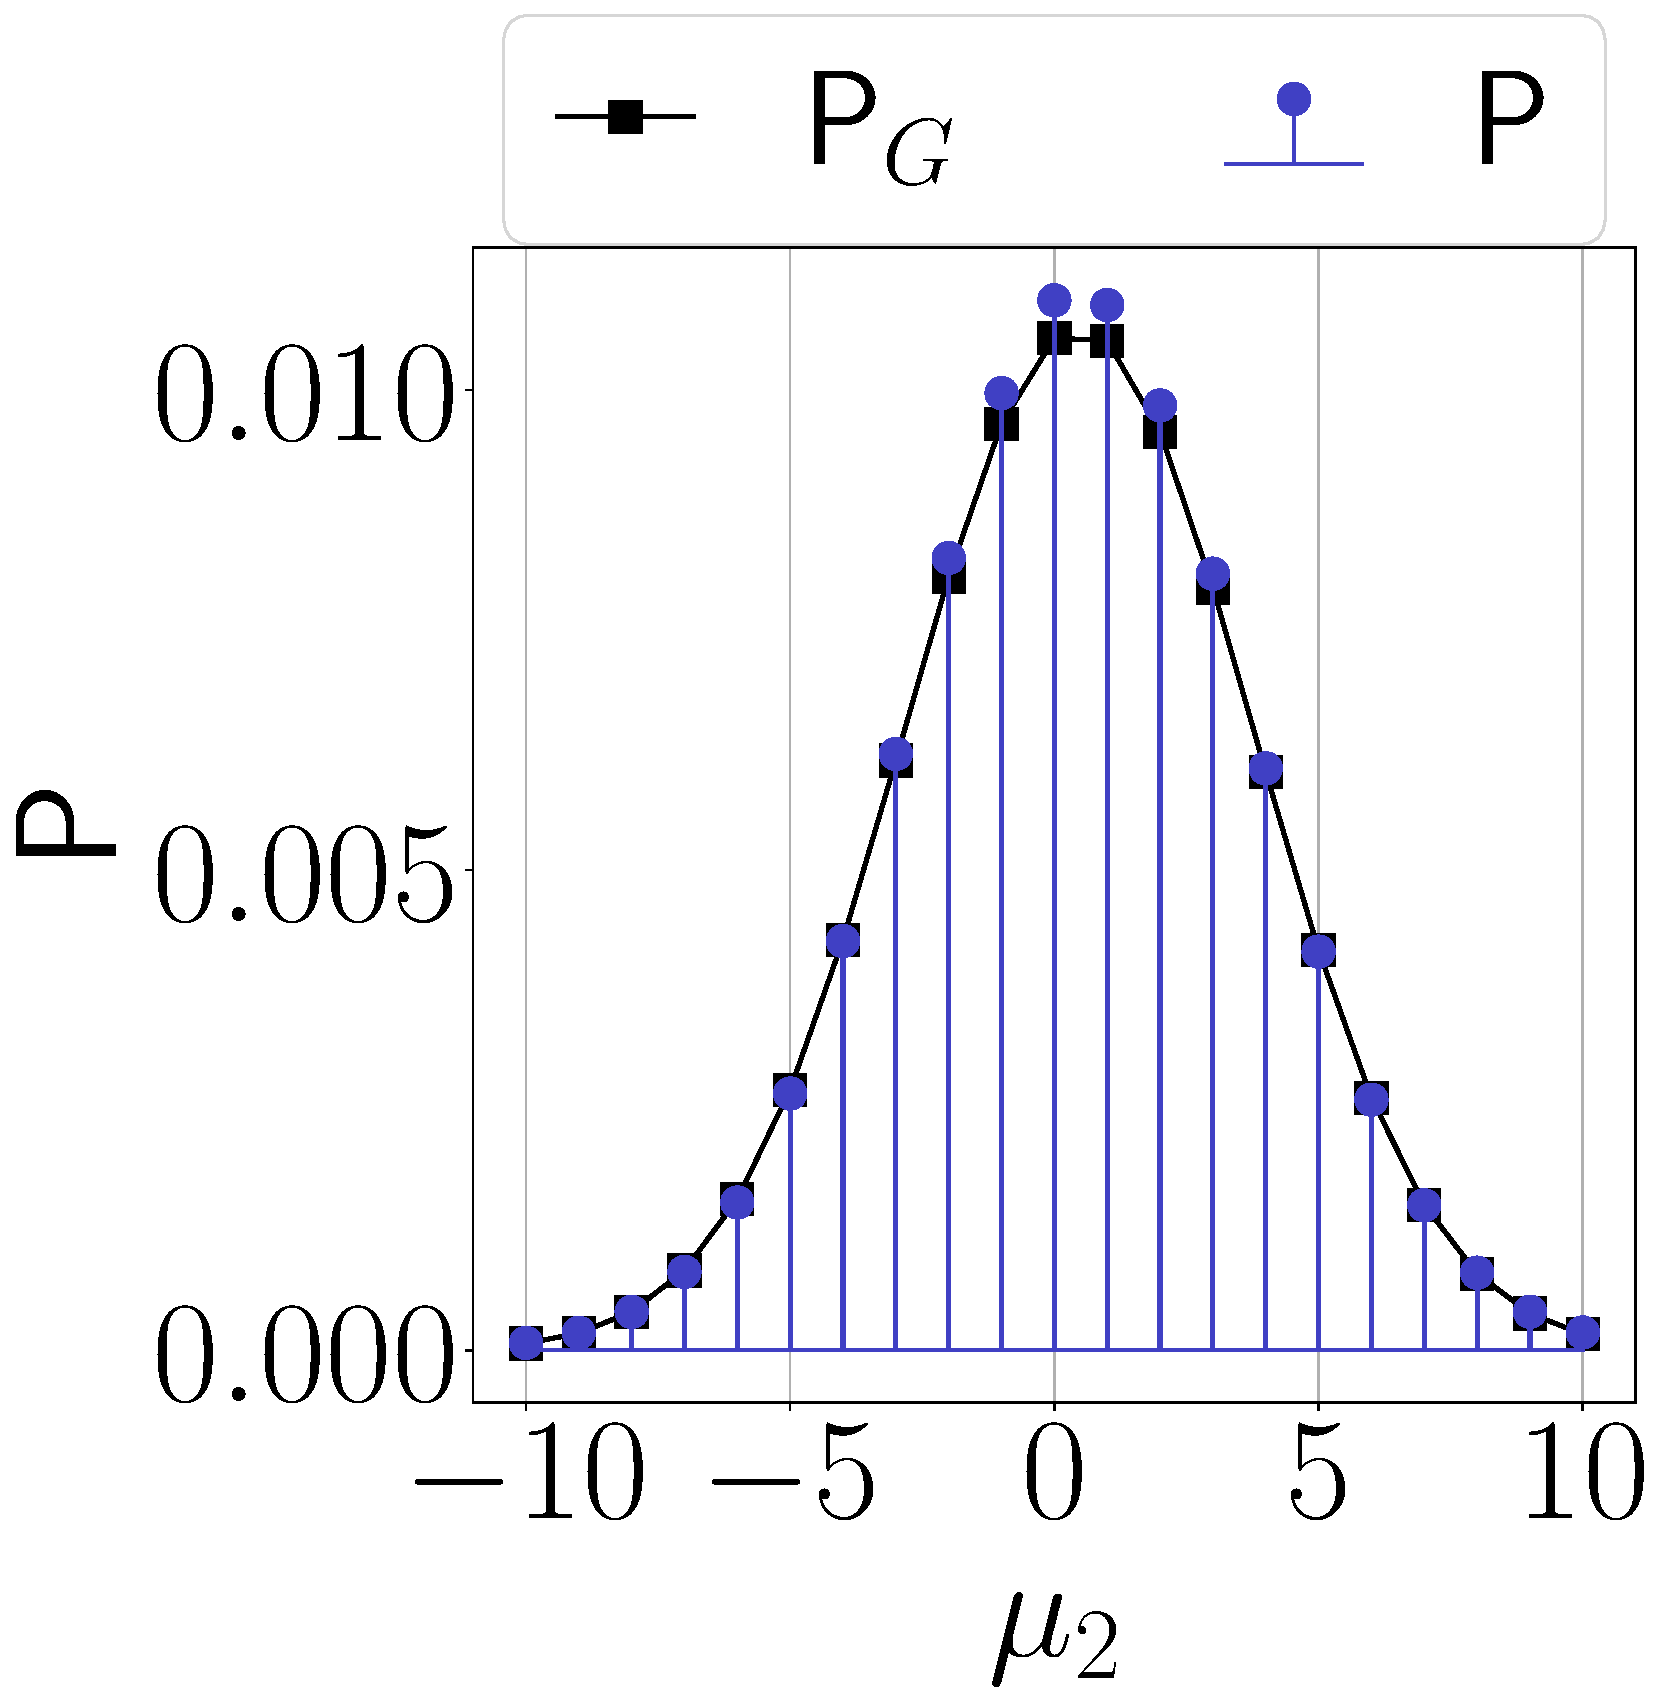
\includegraphics[width=\linewidth]{pics/double-homodyne/dm2.pdf}
\subcaption[]{}
\end{minipage}
    \caption{(a) -- 
     Numerically calculated exact statistical distribution of photon count difference in asymmetrical double homodyne scheme, given by  Eq.~\eqref{eq:accurate-dh}, and calculated distance between this distribution and approximate distribution, given by Eq.~\eqref{eq:Pgood-dh}; (b), (c) -- Projections of exact (blue) and approximate (black) statistical distributions of photon count difference, all calculated for parameters $\alpha=0.25+0.25i$, $\alpha_L=5$, $\eta_1=\eta_3=1$ and $\eta_2=\eta_4=0.75$.
    }\label{fig:dh-statistics}
\end{figure}